
\chapter{Introduction}

%video surveillance+
%person re-id+
% originates from Multi-Target Multi-Camera Tracking 
%open world / closed world+
%face : verification/identification
%common aspects: detection , processing, recognition
%deep learning

%retrieval
%fine-grained recognition
%adaptation

%datasets (cut from the papers) + table with reid dataset?
%architectures
%definitions?
%contribution - what is done

\section{Context}
Today, large-scale distributed multi-camera surveillance systems are installed in many kinds of public places. While such systems are usually provided with an infrastructure to capture, store and access video data, up to this time, the work of watching and searching through such data has been mostly assigned to human operators. The growing amount of surveillance data makes its manual handling non-scalable. The situation has started to change recently with the development and adoption of methods for visual recognition. %todo what is working now in practice?
In particular, recognition of humans (either based on an image of a face or full body) is one of very demanded directions in the surveillance field. An ability to automatically retrieve and compare human images is central for a wide range of applications from long-term multi-camera tracking, forensic analysis and security to retail, and advertising. 


%verification/identification scenarios for both faces and pedestrians
%different visual ques and difficulties

%\bigskip
%\indent\textbf{Person re-identification}
\subsection{Person re-identification}


\textit{Person re-identification} refers to visually matching pedestrian images captured by multiple cameras with (possibly) non-overlapping views. In more detail, it is usually formulated as the task of matching the query (or probe) image to a set of images, called \textit{gallery}. 

For this task, clothing is considered to be the primary source of visual information, whereas faces are assumed to be indistinguishable due to low resolution, or not visible due to individual body positions.  

The main confounding factors of this task stem from the notoriously high variation of the appearance of the same person (even at short time spans) due to differences in pose, camera viewpoint, illumination, and background clutter presence. Examples of typical person re-identification data are shown in \fig{cuhk03_market}.

%%%%%
Most often, person re-identification is formulated as follows:

\begin{problem}
\label{pr:identification}
  \problemtitle{Re-identification}
  \probleminput{Query image $q$, gallery images $G=\{g_i\}_{i=1}^{n_G}$}
  \problemquestion{Find such an image $g_j \in G$ from the gallery that $g_j$ depicts the same identity as $q$: $l_q = l_{g_j}$}
\end{problem}


%check real scenarios for this? multicamera tracking?
There are two main scenarios for the task \citep{zheng2016person}:
\begin{itemize}
\item in the \textit{closed-set} scenario, the gallery has to contain at least one image for every query identity,
\item the \textit{open-set} scenario is more challenging and admits situations when the query identity is not present in the gallery. 
\end{itemize}
The latter implies that the system should be able to decide whether the query identity is contained in the gallery set at all. 
By the time of publishing the results presented in this work, person re-identification performance was rather low even for the closed-set protocols, so much research effort has been first dedicated to improving the results in this setting. Consequently, most of the re-identification benchmark datasets are developed and used for evaluation within the closed-set framework. This work also falls under this category and use the closed-set scenario for evaluation.


\begin{figure}
\begin{center}
\begin{tabular}{ccc}
\begin{tabular}{cccc}

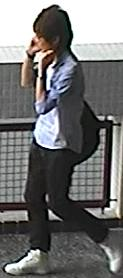
\includegraphics[ height=3cm, width=1.2cm]{Figures/datasets/cuhk03/240_1.jpg}&
%\hspace*{-0.2cm}
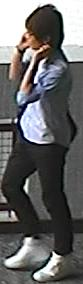
\includegraphics[ height=3cm, width=1.2cm]{Figures/datasets/cuhk03/240_2.jpg}&
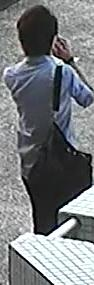
\includegraphics[ height=3cm, width=1.2cm]{Figures/datasets/cuhk03/240_3.jpg}&
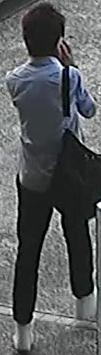
\includegraphics[ height=3cm, width=1.2cm]{Figures/datasets/cuhk03/240_4.jpg} \\
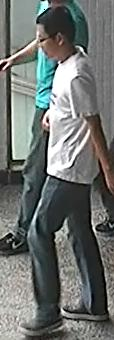
\includegraphics[ height=3cm, width=1.2cm]{Figures/datasets/cuhk03/51_1.jpg}&
%\hspace*{-0.2cm}
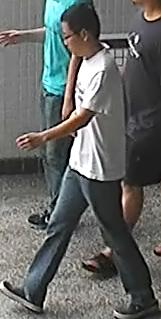
\includegraphics[ height=3cm, width=1.2cm]{Figures/datasets/cuhk03/51_2.jpg}&
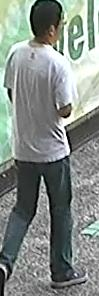
\includegraphics[ height=3cm, width=1.2cm]{Figures/datasets/cuhk03/51_3.jpg}&
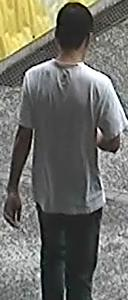
\includegraphics[ height=3cm, width=1.2cm]{Figures/datasets/cuhk03/51_4.jpg} \\
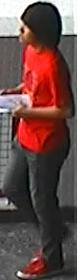
\includegraphics[ height=3cm, width=1.2cm]{Figures/datasets/cuhk03/712_1.jpg}&
%\hspace*{-0.2cm}
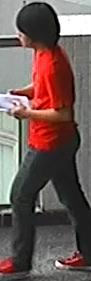
\includegraphics[ height=3cm, width=1.2cm]{Figures/datasets/cuhk03/712_2.jpg}&
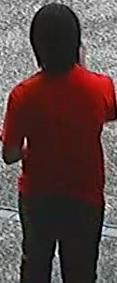
\includegraphics[ height=3cm, width=1.2cm]{Figures/datasets/cuhk03/712_3.jpg}&
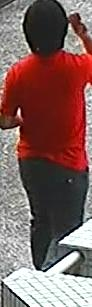
\includegraphics[ height=3cm, width=1.2cm]{Figures/datasets/cuhk03/712_4.jpg} \\

\end{tabular} &   &
\begin{tabular}{cccc}

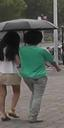
\includegraphics[ height=3cm, width=1.2cm]{Figures/datasets/market-1501/0422_1.jpg}&
%\hspace*{-0.2cm}
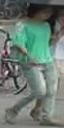
\includegraphics[ height=3cm, width=1.2cm]{Figures/datasets/market-1501/0422_2.jpg}&
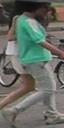
\includegraphics[ height=3cm, width=1.2cm]{Figures/datasets/market-1501/0422_3.jpg}&
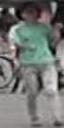
\includegraphics[ height=3cm, width=1.2cm]{Figures/datasets/market-1501/0422_4.jpg} \\

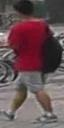
\includegraphics[ height=3cm, width=1.2cm]{Figures/datasets/market-1501/1059_1.jpg}&
%\hspace*{-0.2cm}

\includegraphics[ height=3cm, width=1.2cm]{Figures/datasets/market-1501/1059_2.jpg}&

\includegraphics[ height=3cm, width=1.2cm]{Figures/datasets/market-1501/1059_3.jpg}&
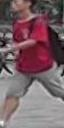
\includegraphics[ height=3cm, width=1.2cm]{Figures/datasets/market-1501/1059_4.jpg} \\


\includegraphics[ height=3cm, width=1.2cm]{Figures/datasets/market-1501/0425_1.jpg}&
%\hspace*{-0.2cm}

\includegraphics[ height=3cm, width=1.2cm]{Figures/datasets/market-1501/0425_2.jpg}&

\includegraphics[ height=3cm, width=1.2cm]{Figures/datasets/market-1501/0425_3.jpg}&
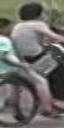
\includegraphics[ height=3cm, width=1.2cm]{Figures/datasets/market-1501/0425_4.jpg} \\


\end{tabular}\\
(a)&    & (b)
\end{tabular}


    \caption{Sample images of publicly available person re-identification datasets (a) - CUHK03 dataset~\citep{Li14}, (b) - Market-1501 dataset~\citep{zheng2015scalable}. In each group, each row corresponds to a person, different camera views are shown for each identity. The data demonstrate  variations in pose, illumination, background and the presence of clutter}.
    \label{fig:cuhk03_market}
\end{center}
\end{figure}

In most of person re-identification datasets, the training images are usually captured during limited time within middle-size camera networks. This is due to a large amount of manual effort required to analyze such data to find occurrences of the same person across different camera views.
Therefore, commonly, each identity has a relatively small amount of different images (in the order of $10$).



%todo difficulties of real world applications: large amount of data, open set?... practical issues for reid

%\bigskip
%\indent\textbf{Face recognition}
\subsection{Face recognition}
\label{sect:face}
%face identification vs verification
\textit{Face recognition} also refers to the task of matching human images. But in contrast to person re-identification, faces are matched instead of full-body images.
There are also two main scenarios for face recognition \citep{jafri2009survey}:
\begin{itemize}
\item \textit{face identification} describes one-to-many matching, when an image of an unknown individual is compared to a database of images of known individuals in order to determine this person's identity. For example, checking the person's access level may require searching for this person in the employee database. 
\item \textit{face verification} describes one-to-one matching when, given a pair of face images, one should determine whether they depict the same identity. For example, this case can be useful to ensure that the person is the individual he/she claims to be.
\end{itemize}

The formulation for face identification is similar to \pr{identification}, whereas face verification is:

\begin{problem}
\label{pr:verification}
  \problemtitle{Verification}
  \probleminput{A pair of images $(q_1, q_2)$}
  \problemquestion{Determine whether the images $q_1$ and $q_2$ depict the same person or two different persons: 
                   $l_{q_1} ?= l_{q_2}$}
\end{problem}


Similarly to person re-identification, the difficulties of the task come from the uncontrolled environment, \eg{} variations in pose, lighting, different facial expressions and hairstyle.
However, unlike person re-identification, recent face recognition works have been more focused on higher quality images that are often taken by professional photographers, rather than surveillance systems. Mainly, this is due to the fact that face recognition is not limited to only surveillance-based applications. Moreover, it is a challenging task even in the case of sufficient image quality: many methods are aimed at extracting important facial information, while ignoring irrelevant variations (\eg{} \citep{Chopra05,parkhi2015deep,SchroffKP15}). Another circumstance can be mentioned: it is now possible to use multiple publicly available Internet resources to extract images of well-known persons (\eg{} actors, politicians) using their names as queries to a search engine. Therefore large training datasets for face recognition can be harvested from the Internet, where lots of face images with known identities of people in them can be mined in an automatic or semi-automatic way \citep{parkhi2015deep}. When trained on such datasets, deep face recognition networks are rivaling and exceeding human face recognition performance, when applied to similar types of images. 

%todo : many images for the same person
Yet, many, perhaps majority, of practical scenarios require building vision systems that recognize faces in images that are quite different from those harvested from the Internet. These scenarios include surveillance for security purposes, smart home applications, collaborative robotics, which all come with specific camera parameters, camera positioning, lighting conditions that are all quite different and are often of much lower quality than face images typically encountered on the Internet.  %In this work, I investigate and compare approaches to building face recognition systems that can operate under this strong domain shift, being able to leverage large annotated datasets of Internet face images and videos for the efficient recognition of faces in surveillance data. 


%to do image/video reid/face

%\bigskip
%\indent\textbf{Image retrieval}
\subsection{Relation to image retrieval and classification}
%todo check the intuition in the israel paper about faces!
%relation to classification and retrieval?
%something about application of classification losses/deep nets etc.

For both human recognition problems, the training data most often consist of some number of training images along with their identities. This makes the tasks quite similar to classification, given that each identity corresponds to one class. Although in practice, such recognition and re-identification systems, once trained, are required to work for a large number of unseen identities. Therefore in most of the evaluation protocols, test and train data contain non-overlapping sets of identities. 

The discussed property of the tasks is also inherent to general image retrieval. The latter also requires the recognition system to be able to estimate the similarity between images of probably unseen classes and, therefore, to capture the notion of similarity from the training data and generalize it. 

%\bigskip
%\indent\textbf{The key problem}
\subsection{The key problem}
For both of the described human recognition problems, the recognition step follows several other  preprocessing steps: face/full-body detection and, possibly, alignment (although some works include the alignment step into recognition, \eg{} \citep{Tadmor2016LearningAM}). This work is focused on the recognition step. 

While various scenarios for person re-identification and face recognition exist, at a high level, the key task for both problems can be informally defined as follows: 


\begin{problem}
\label{pr:similarity_estimation}
  \problemtitle{Similarity estimation}
  \probleminput{A pair of images $(q_1, q_2)$}
  \problemquestion{
    to measure the similarity value for $(q_1, q_2)$ in such a way that a pair would get:
    \begin{itemize}
        \item high similarity score in case of depicting the same person (such pairs are also called \textit{positive} pairs),
        \item low score in case of depicting different persons (\textit{negative} pairs). 
    \end{itemize}}
\end{problem}

% \textbf{to measure the similarity for pairs of images in such a way that a pair would get}:
% \begin{itemize}
%     \item high similarity score in case of depicting the same person (such pairs are also called \textit{positive} pairs),
%     \item low score in case of depicting different persons (\textit{negative} pairs). 
% \end{itemize}


This requires to construct a robust representation and an appropriate similarity measure which would facilitate assigning corresponding similarity scores.


%check facenet for explanation
%ranking vs metric learning


%todosiamese sharing weights, siamese not sharing weights?




%\bigskip
%\indent\textbf{General approaches to human recognition}
\subsection{General approaches to human recognition}

%todo mention eigen fisher face and other holistic approaches for faces
Traditionally, features/representation design and fixed distance/similarity function design have been considered as two separate steps in building the recognition system. Consequently, most of the research efforts on face recognition and person re-identification have been dedicated to these two problems. Some works focused on finding a discriminative representation \citep{ma2012bicov, ma2012local, DBLP:journals/cviu/BazzaniCM13}. Others sought for a special transformation of a fixed feature space in order to improve the retrieval quality \citep{hirzer2012person,mignon2012pcca}, or the quality of metric-based algorithms, like nearest neighbor classification \citep{weinberger2009distance}. Most of the works under this category formulate the task as Mahalanobis metric learning. The idea behind it is to learn a linear transformation to a new feature space where Euclidean distance can be used in order to solve \pr{similarity_estimation}. The non-linear case is achieved by using the 'kernel trick'. Some approaches aimed at both feature design and metric learning \citep{liao2015person}.

% turn to neural networks.
Unlike the mentioned approaches, deep neural networks allow to learn a hierarchy of representations with different levels of abstraction. Starting from the most low-level representations that can be extracted using the first layers of the network, the task-specific information becomes more and more distilled while forwarding through a trained deep neural network. Thus deep neural networks are able to combine the two steps of feature extraction and learning a prediction model based on such features, allowing to automatically find more suitable feature extractors for a particular task. For example, in human recognition, the deep learning approach may help to take into account important clothing parts or facial features and at the same time discard the illumination and pose variations to some extent.

Deep learning methods have improved state of the art in multiple visual recognition tasks, including face recognition \citep{Taigman14,parkhi2015deep,SchroffKP15}. The situation has been rather different for person re-identification:  until recently, the results of some traditional methods \citep{paisitkriangkrai2015learning} were still better than those of the first deep learning approaches to person re-identification \citep{Li14}. 

Therefore, one goal of this work, among others, is to consider deep learning methods for the person re-identification task and try to improve over the non-deep methods. 


%todo picture
\section{Objectives and motivation}

The goal of this work is to explore building deep learning systems for human recognition.

In particular, the development of perhaps every deep recognition system includes several important tasks: 
\begin{itemize}
    \item the architecture design,
    \item the objective function design,
    \item the choice of training data.
\end{itemize}
%has contitued?
To a certain extent, each of these tasks constitutes a challenge in the context of human recognition. The presence of a large domain shift between the training and test data (\eg{} when using different sets of cameras) is also a serious problem for both tasks of person re-identification and face recognition as it may cause a considerable performance drop.

In the remainder of this section, each of the three aspects is discussed to build a foundation for the ideas that are presented in the subsequent chapters: \chapt{hist} addresses the objective function design for similarity learning, \chapt{bilinear} considers the architecture design for person re-identification, \chapt{gradrev} and \chapt{wildface} address domain adaptation for person re-identification and surveillance face recognition. 


\subsection{Approaches to building CNNs for human recognition}
\label{sect:intro_siamese}

\begin{figure}
\begin{tabular}{cc}
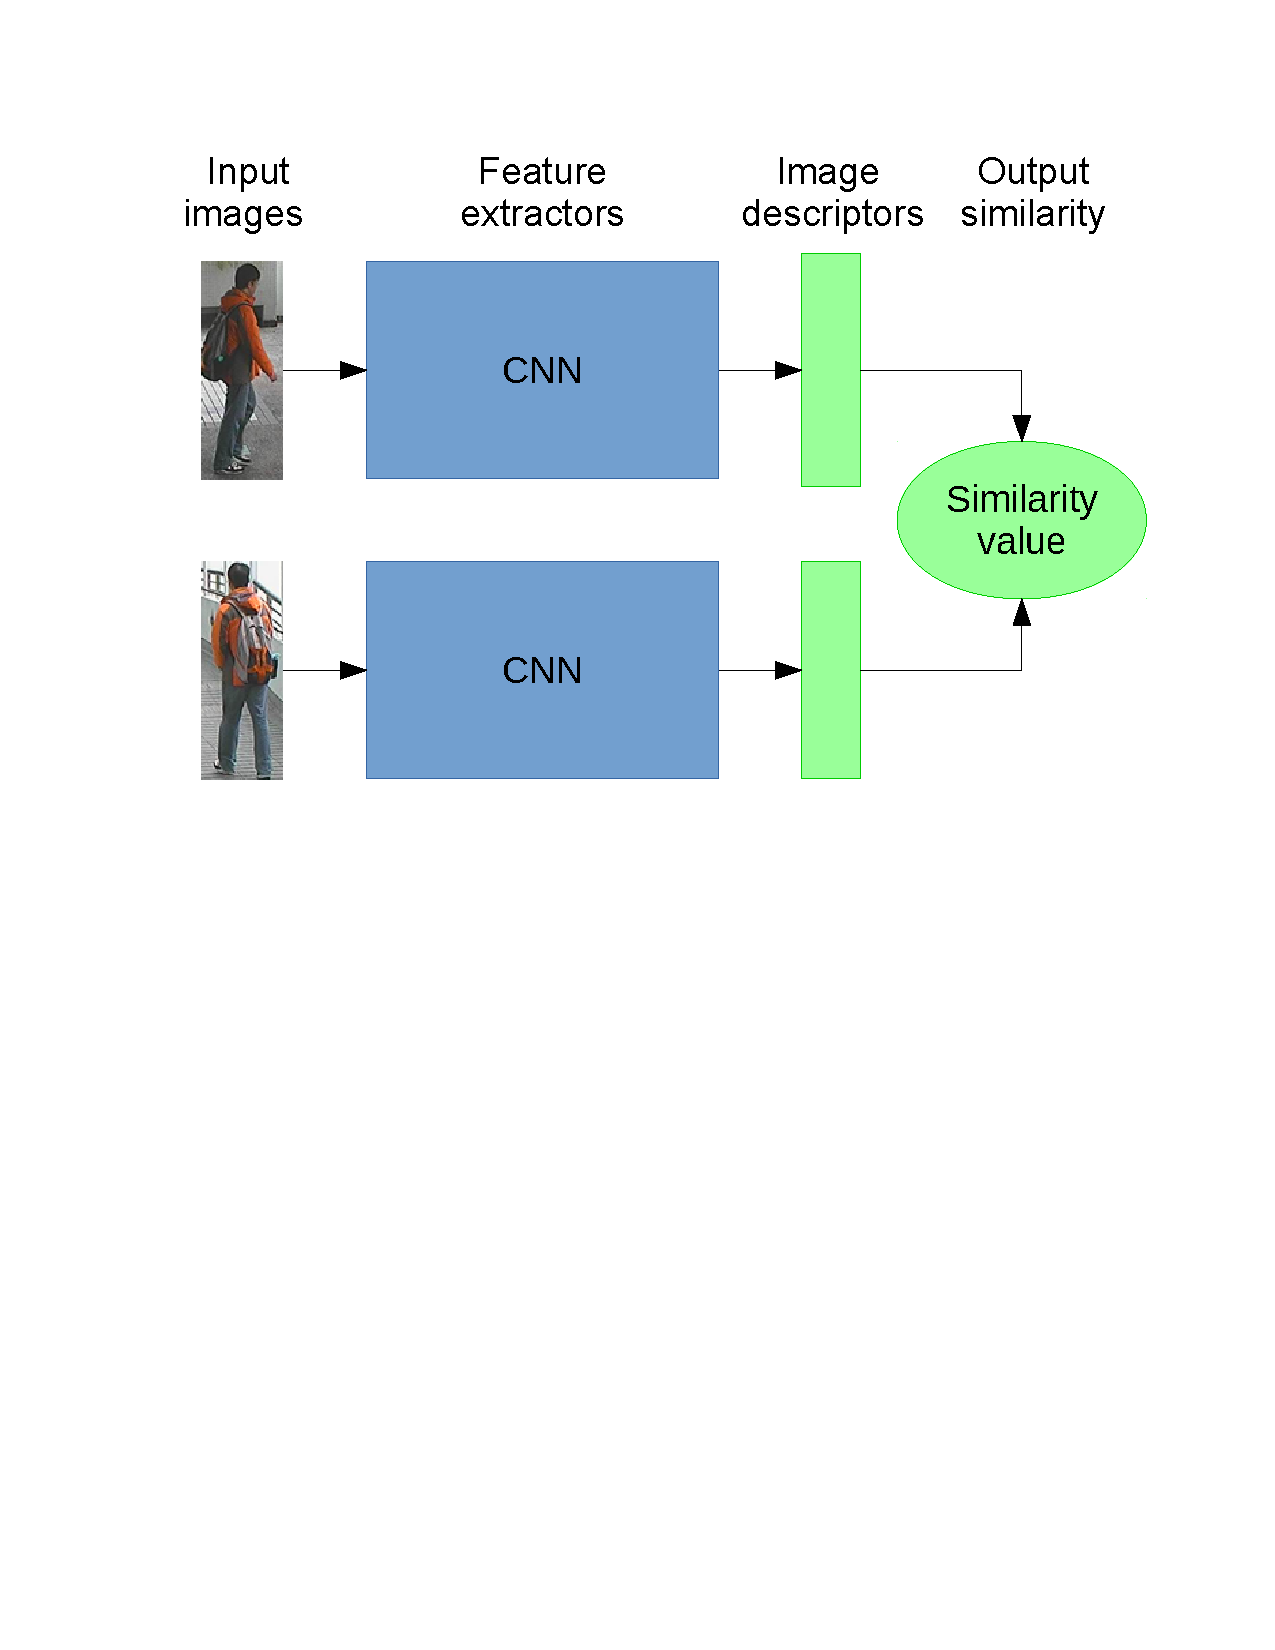
\includegraphics[width=0.47\linewidth, height=5cm]{Figures/siamese.pdf}&
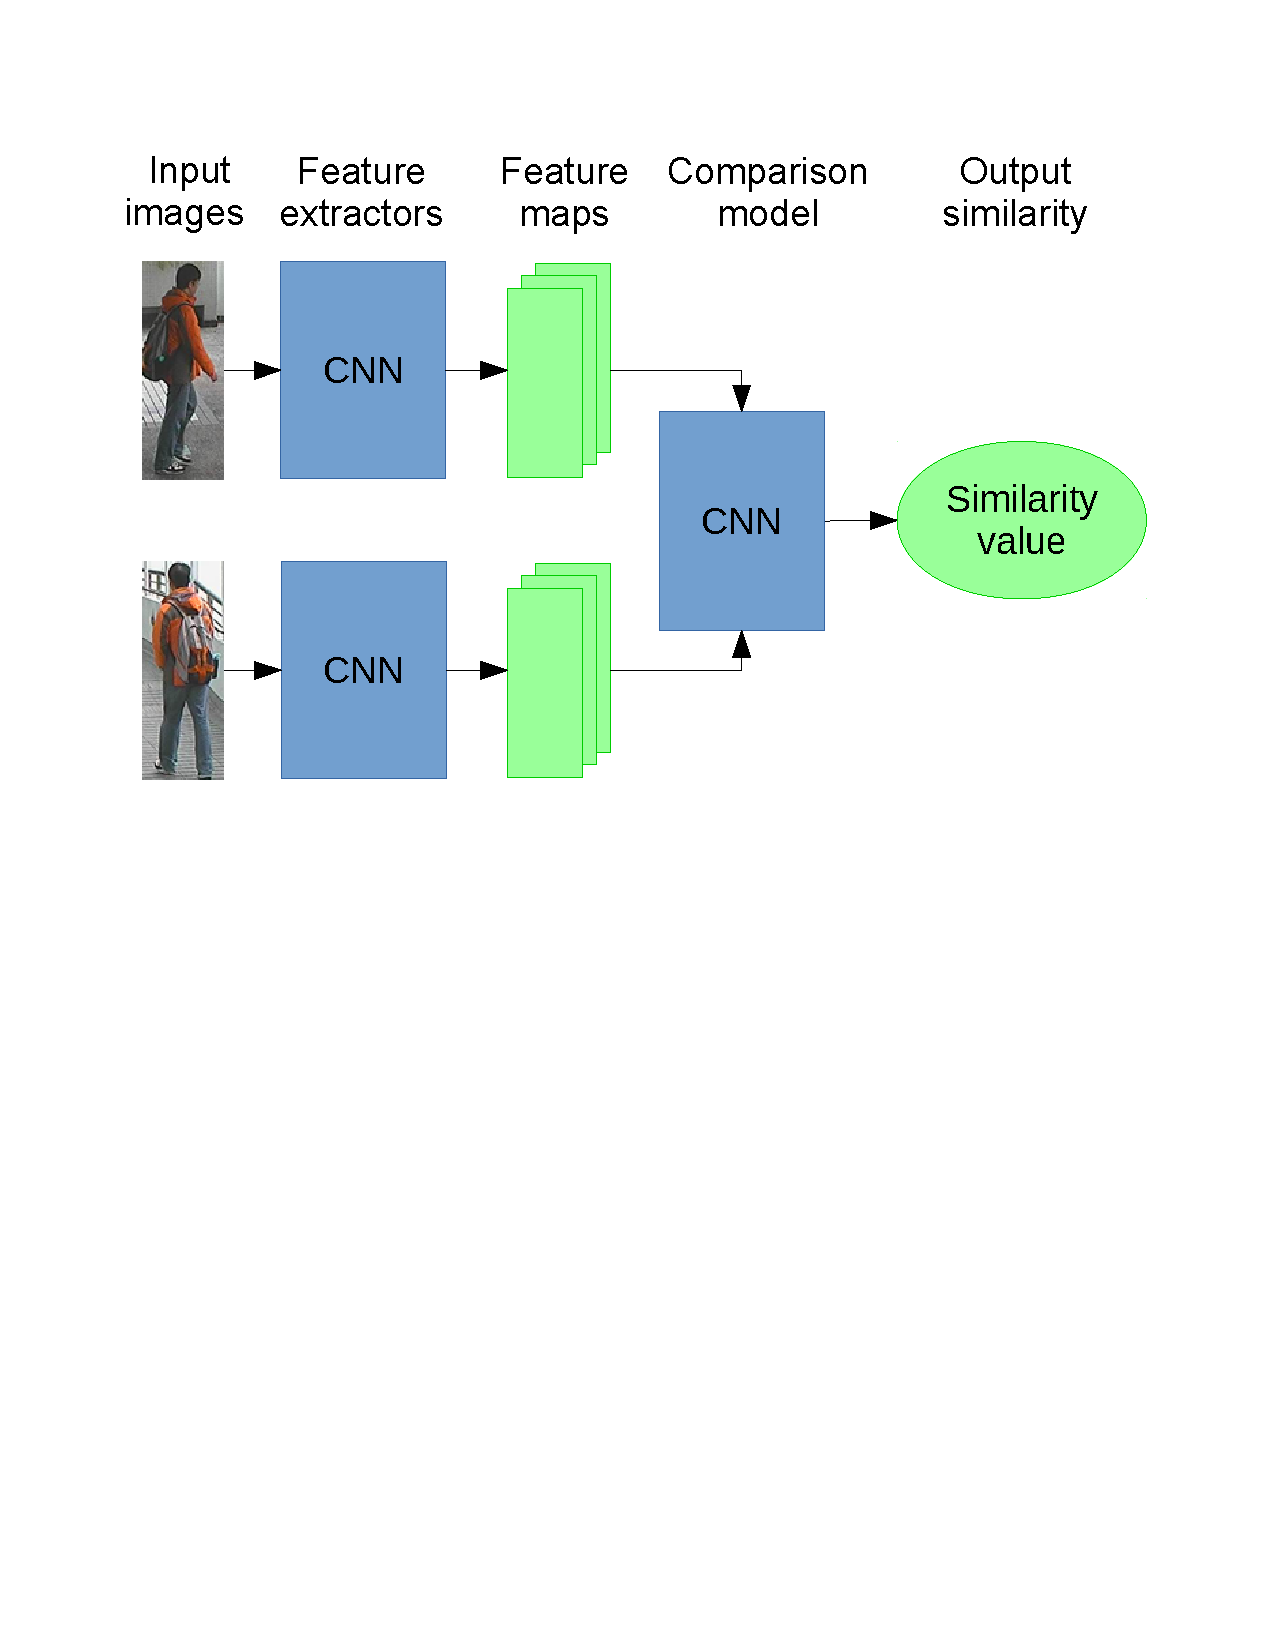
\includegraphics[width=0.50\linewidth, height=5cm]{Figures/siamese2.pdf}&
\\
(a) & (b)
\end{tabular}

\caption{(a) - A general siamese architecture \citep{Bromley93, Chopra05} scheme: two images are first mapped into a descriptor space, the similarity value is computed as a function of a pair of output descriptors; most often, negative Euclidean distance or cosine function is used as a simple similarity measure. (b) - A modification of a siamese architecture, where the similarity value is computed using an additional CNN (convolutional neural network), so the difference of images is  more explicitly modeled than in the original siamese architecture.}
\label{fig:siamese}
%todo fix the picture

\end{figure}

Deep learning allows to learn feature extractors so that their parameters are optimized for a particular task. 
\textit{Siamese} architecture, that was initially suggested for signature verification by \citep{Bromley93}, is a standard deep learning approach to retrieval problems. It typically consists of two identical subnetworks that parametrize a mapping from an image space to a descriptor space. The siamese architecture is usually trained in such a way that Euclidean or angular distance between the descriptors reflects the similarity and dissimilarity of corresponding images.
For example, \citep{Yi14, parkhi2015deep} utilize the siamese architecture for person re-identification and face verification correspondingly.

At the same time, some other methods modify the approach to explicitly model the differences of image regions at multiple feature levels \citep{ahmed2015improved,Li14,chen2016deep}. Such architectures map a pair of images directly to a scalar similarity score and therefore a complex pairwise similarity function is learned instead of per-image embeddings. However, such approaches require multiple pairwise forward operations at test time: a query image should be compared to each of the gallery images by computing the similarity score with a trained neural network. Generally, this is much slower than computing pairwise Euclidean/angular distances for a number of pre-computed descriptors. The described variants are shown in \fig{siamese}.

Therefore this work builds on top of more standard siamese approaches in order to learn a mapping to a descriptor space so that simple similarity measures can be applied to the resulting descriptors.

%such as those used for image classification or face embedding
However, the choice of the convolutional architecture for embedding in the case of person re-identification is far from obvious. In particular, existing ``standard'' architectures that combine convolutional layers followed by fully-connected layers can fail to achieve sufficient invariance to strong viewpoint changes as well as to non-rigid articulations of pedestrians, given the limited amount of training data typical for re-identification tasks and datasets. 

\chapt{bilinear} describes a person re-identification architecture that is based on the idea of bilinear convolutional networks (Bilinear CNNs) \citep{lin2015bilinear} that were originally presented for fine-grained classification tasks and later evaluated for face recognition \citep{roychowdhury2015face}. At the same time, the suggested architecture is built on top of the siamese neural network earlier suggested by \citet{Yi14} for person re-identification. It is shown to perform favorably for three publicly available person re-identification datasets, for two largest of them, state-of-the-art results were achieved (on the moment of publication).



\subsection{Objective functions for training siamese architectures}
\sect{intro_siamese} describes the principle of siamese neural networks. The goal of training such architectures is to build a mapping from an image space to a high-dimensional descriptor space. Such descriptors are also called \textit{embeddings}. If similar images are mapped into points that are close in the descriptor space, and non-similar - to points that are far away from each other, the image similarity can be estimated by the distance in the descriptor space. In order to learn such mapping, a certain objective should be defined. It should encourage the proximity of embeddings of similar images and discourage it for dissimilar images. 

%, the use of approximate search methods, and ultimately lead to faster and more scalable systems. 

Learning deep feed-forward embeddings still poses a challenge. While it is possible to write down a loss based on tuples of training points expressing the above-mentioned objective, optimizing such a loss rarely works ``out of the box'' for complex data. This is evidenced by the broad variety of losses, which can be based on pairs, triplets or quadruplets of points.  Most of the existing losses come with a certain number of tunable parameters, and the quality of the final embedding is often sensitive to them.%, as well as by a large number of optimization tricks employed in recent works to reach state-of-the-art, such as pretraining for the classification task while restricting fine-tuning to top layers only~\citep{Taigman14,parkhi2015deep}, combining the embedding loss with the classification loss~\citep{Sun14}, using complex data sampling such as mining ``semi-hard'' training triplets \citep{Schroff15}. Most of the proposed losses and optimization tricks come with a certain number of tunable parameters, and the quality of the final embedding is often sensitive to them.


A new objective function for training deep embeddings is suggested in \chapt{hist}. It is based on pairwise training data and does not incorporate usual hyper-parameters that require careful tuning for different datasets.   %This loss function aims at pushing apart the similarity values for positive and negative pairs: positive pairs should have higher similarity values for better retrieval (so, assumption \ref{assumption_1} is used here). 
%However, instead of comparing the similarity values for separate pairs, the loss operates on the level of distributions of such similarity values.
This loss is computed in two steps: first, the two similarity distributions for positive and negative pairs are estimated, second, their overlap is computed. The goal is to minimize such overlap, so that positive pairs have higher similarity than negative pairs. The experimental section of \chapt{hist} shows that the suggested loss outperforms several other point-based losses for person re-identification and also performs well for several other retrieval problems. 


\subsection{Different domains in human recognition}


\newlength\reidheight
\setlength{\reidheight}{2.5cm}
\addtolength{\tabcolsep}{-3pt}
\begin{figure*}
\centering
\begin{tabular}{cccc|cccc|cccc}
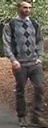
\includegraphics[height=\reidheight]{Chapters/gradrev/figures/dataset_samples/viper/a/000_45.png}&

\includegraphics[height=\reidheight]{Chapters/gradrev/figures/dataset_samples/viper/b/000_45.png}&
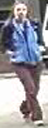
\includegraphics[height=\reidheight]{Chapters/gradrev/figures/dataset_samples/viper/a/001_45.png}&

\includegraphics[height=\reidheight]{Chapters/gradrev/figures/dataset_samples/viper/b/002_90.png}&
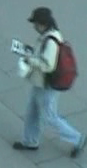
\includegraphics[height=\reidheight]{Chapters/gradrev/figures/dataset_samples/PRID/a/img_0001.png}&
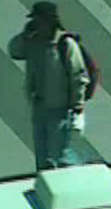
\includegraphics[height=\reidheight]{Chapters/gradrev/figures/dataset_samples/PRID/b/img_0001.png}&
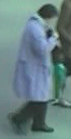
\includegraphics[height=\reidheight]{Chapters/gradrev/figures/dataset_samples/PRID/a/img_0002.png}&
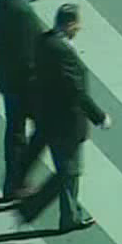
\includegraphics[height=\reidheight]{Chapters/gradrev/figures/dataset_samples/PRID/b/img_0003.png}&
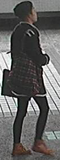
\includegraphics[height=\reidheight]{Chapters/gradrev/figures/dataset_samples/cuhk/a/001_00005.png}&
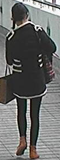
\includegraphics[height=\reidheight]{Chapters/gradrev/figures/dataset_samples/cuhk/b/001_00221.png}&
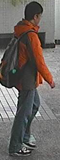
\includegraphics[height=\reidheight]{Chapters/gradrev/figures/dataset_samples/cuhk/a/002_00280.png}&
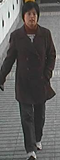
\includegraphics[height=\reidheight]{Chapters/gradrev/figures/dataset_samples/cuhk/b/003_00403.png}\\
\multicolumn{4}{c}{VIPER}&
\multicolumn{4}{c}{PRID}&
\multicolumn{4}{c}{CUHK}
\end{tabular}
\caption{Matching and non-matching pairs of probe-gallery images from different person re-identification datasets. The three datasets are treated as different domains in our experiments.}
\label{fig:reidsamples}
\end{figure*}


%intro
%Since the time when the first deep learning approaches for person re-identification started to appear, the results have improved (\citep{something cool}) significantly. Many visual recognition tasks benefited from the development of new powerful architectures (\citep{resnet}) including person re-identification (\citep{}). The results for face recognition exceeded the human performance even earlier (\citep{the paper that exceeds human performance}).



%problem
Cross-domain human recognition remains a hard problem for many practical scenarios. 
For person re-identification, the common case considered in literature is training and testing on the data obtained from different sets of cameras. Given the fact that different re-identification benchmark datasets were collected separately and independently, they are very suitable for modeling such use case. Indeed, pedestrian images differ considerably between some publicly available datasets. Such difference may come from the different illumination conditions, background, resolution and position of cameras. The examples of three different person re-identification datasets are shown in \fig{reidsamples}.

\chapt{gradrev} demonstrates that the performance of cross-domain person re-identification can be improved by domain-adversarial training. This method is initially developed for cross-domain classification problems and is also described in \chapt{gradrev}. Eight domain pairs are used for evaluation, where each of the domains corresponds to one of tree popular re-identification datasets. 

An important cross-domain case of person re-identification is considered in \chapt{wildface}. As it was mentioned in \sect{face}, the large-scale training data for face recognition are usually harvested from the Internet and are characterized by much higher quality then surveillance data. In \chapt{wildface}, it is demonstrated how surveillance face recognition can be approached using recent image-to-image translation techniques. The domain-adversarial training method introduced in \chapt{gradrev} is also included in the evaluation.

%something about gradrev

%My contribution to \chapt{gradrev} lies in demonstration that the suggested domain adaptation approach is also applicable to retrieval tasks, like person re-identification, where the task-specific label predictor is replaced by a siamese subnetwork. 


 %Still, to the best of our knowledge, there are no works approaching face recognition for surveillance data.

%about the face chapter

\section{Datasets}

In this section, we describe several publicly available person re-identification and face verification datasets that are used in this work. Person re-identification datasets are used for training and evaluation. Face verification datasets are mostly used as training data for  surveillance face verification. The specially collected surveillance data are used for evaluation and described in \chapt{wildface}.




\begin{itemize}

    \item  PRID \citep{Hirzer_h.:person} contains images of $385$ persons viewed from camera A and images of $749$ persons viewed from camera B,  $200$ persons appear in both cameras. $100$ persons appearing in both camera views are used for training. The images of the other $100$ persons from camera A are used as probe, all images from camera B excluding those used in training ($649$ in total) are used as gallery at test time. 
    
    \item VIPeR \citep{Gray07evaluatingappearance} also contains images taken with two cameras, and in total $632$ persons are captured, for every person, there is one image for each of the two camera views. Images of $316$ identities are used for training and all others for testing.
    
    \item CUHK01 \citep{LiZW12} contains images of $971$ identities from two disjoint camera views. Each identity has two samples per camera view. $485$ identities are randomly chosen for training and the other $486$ for test.  
    \item CUHK02 \citep{li2013locally} consists of images from five pairs of cameras, two images for each person from each of the two cameras. It contains images for $1816$ identities in total, but most often, $971$ from the first pair of cameras are used.
    
    \item CUHK03 \citep{Li14} includes $13,164$ images of $1,360$ pedestrians captured from 3 pairs of cameras. The two versions of the dataset are provided: \textit{CUHK03-labeled} and \textit{CUHK03-detected} with manually labeled bounding boxes and automatically detected ones accordingly.  $1,360$ identities are split into $1,160$ identities for training, $100$ for validation and 100 for testing.
    \item Market-1501 \citep{zheng2015scalable} contains $32,643$ images of 1,501 identities, each identity is captured by from two to six cameras. The dataset is randomly divided into the test set of 750 identities and the train set of 751 identities. For each identity in the test set, one image in each camera is selected and used as a query. Manually drawn bounding boxes are used for query images, and automatically detected ones for training images as well as for the gallery images in the test set. 
    Market-1501 also includes ''distractor'' images that correspond to false detections, which makes evaluation on the dataset even more realistic and challenging. Matching is done across different cameras, and in the situation when the gallery images of the same person and form the same camera as the query are ignored and not counted as true positives during the evaluation. 
    \item YouTube Faces (YTF)~\citep{WolfHM11}   consists of $3,425$ videos of $1,595$
 people collected from YouTube, with an average of 2 videos per identity. 
     \item VGG Face \citep{parkhi2015deep} contains $2,6$M images of $2,622$ identities harvested from the Internet. 
 \end{itemize}


Following \citep{Li14}, we use Recall@K metric to report our results for person re-identification. Recall@K (also referred as Cumulative Matching Characteristic curve) is computed for different values of K as a percentage of the queries for which the correct match is found among the first K results, where the results are sorted by similarity to the query.

%todo make more understandable
%At test time single-shot Recall@K curves are calculated for CUHK01 and CUHK03, multi-shot results are calculated for Market-1501. Five random splits are used for both CUHK01 and CUHK03 to calculate the resulting average Recall@K. Some sample images of CUHK03 and Market-1501 datasets are shown in figure \ref{fig:teaser}.

\section{Architectures}
\label{sect:intro_architectures}
\begin{itemize}

    \item Deep Metric Learning (DML) architecture has been suggested in \citep{Yi14} for person re-identification.
    Is is used in \chapt{hist}, \chapt{bilinear} and \chapt{gradrev} as a base architecture.
    The network incorporates independent streams, in which three overlapping parts of person images are processed separately (top, middle and bottom parts), and produces  $500$-dimensional descriptor as an output.
 % These sub-networks are responsible for calculating descriptors for a pair of images which are then connected via distance function.  %Each of the two ``siamese'' sub-networks include three independent streams, in which three overlapping parts of person images are processed separately, namely, the top part (head, upper torso), the middle part (torso), and the lower part (legs, lower torso). This is done in order to take into account different statistics of textures, shapes, and pose changing in different parts of the image, while still utilizing convolutional layers with spatially-invariant kernels. 

 Each of the three streams incorporates two convolutional layers of size $7\times7$ and $5\times5$, followed by the rectified linear (ReLU) non-linearity and max-pooling with the kernel size of two pixels and the stride of two pixels.  500-dimensional descriptor vector is produced as an output of a fully-connected layer, that accepts the outputs of the three convolutional streams. For each training pair of images, the cosine similarity of these descriptors is calculated. %At training time, the similarity value with the pair label (+1 for the same identity, -1 - for different identities) is then fed into the loss function.

 As in \citep{yi2014deep}, we consider the \textit{view-invariant} architecture with the same weights shared for all views in the dataset. This case is more general as the trained networks can be used for new out-of-sample cameras, unlike the view-specific case that lacks weights sharing (which makes networks to capture view-specific appearance peculiarities).
    
    \item VGG-face \citep{parkhi2015deep} is a powerful architecture for face recognition. It is used in \chapt{wildface}. It consists of $5$ blocks of convolution layers. Each block is followed by max-pooling. Three fully-connected layers are inserted at the end, their output dimensions are: $4096$, $4096$ and $2622$. The layer before last is used to extract deep embeddings. 
    
\end{itemize}
%It has three CNN streams for the three parts of the pedestrian image (head and upper torso, torso, lower torso and legs). Each of the streams consists of 2 convolution layers followed by the ReLU non-linearity and max-pooling. The first convolution layers for the three streams have shared weights. Descriptors are produced by the last 500-dimensional inner product layer that has the concatenated outputs of the three streams as an input.



%We use the Deep Metric Learning (DML) architecture proposed by \citep{yi2014deep} as baseline, it is described in \sect{intro_architectures}.

%The CNN proposed by \citep{yi2014deep} incorporates ``siamese'' neural net, initially introduced for signature verification \citep{bromley1993signature} and later for face recognition in \citep{chopra2005learning}. The siamese architecture consists of two similar sub-networks for separate processing of two input images. 
%

\section{Contribution}

This work presents the following contributions:
\begin{itemize}

    \item
    The work presents a new loss function for training similarity-based siamese neural networks. Such training is performed to build a mapping from an image to a descriptor space so that semantically similar images are close to each other and non-similar images are distant in this descriptor space. Compared to the existing (by the time of publication) loss functions (\eq{bindev}), the suggested loss does not incorporate special hyper-parameters, like thresholds for separating the pairs of matching images from the pairs of non-matching images. At the same time, it is based on the pairwise training and therefore does not require more complex forms of training data, like triplets or quadruplets. The experiments are performed for the two largest person re-identification datasets (the suggested loss function performed best among several others: \eq{bindev}, \eq{triplet}, \eq{eq:lifted}) and for two datasets for other retrieval problems (second-best result). This contribution is the subject of \chapt{hist} and published as \citep{UstinovaNIPS16}. 

    \item
    A novel architecture for person re-identification is suggested in \chapt{bilinear}. This chapter also offers an analogy between person re-identification and fine-grained recognition problems. This analogy allows to build upon the Bilinear CNN model of \citep{lin2015bilinear} and adapt it to the task: the suggested approach can be considered as a middle ground between Bilinear CNNs and regular models. The suggested architecture is shown to outperform several baselines on three popular person re-identification benchmarks. For the two largest datasets, the state-of-the-art results were achieved (on the moment of publication). The results of this part are published as \citep{ustinova2017multi}.
 
    \item
    %todo: presented in chapter???
    The deep feature-level domain adaptation model \citep{ganin2016domain} is demonstrated to be applicable to person re-identification. The modification of domain-adversarial learning, also described in \chapt{gradrev}, lies in replacing the task-specific label predictor by a siamese subnetwork that maps pedestrian images into a descriptor space. This contribution is presented in \chapt{gradrev} and published as a part of the work \citep{ganin2016domain}. The experiments are conducted for eight domain pairs. In these domain pairs, the source and target domains are represented by two (of three in total) different publicly available person re-identification datasets. Thus, the practical situation of the domain shift between different sets of cameras is considered.

    \item
    Face recognition in the presence of a strong domain shift is considered in \chapt{wildface}. Pixel-level domain adaptation approach based on the CycleGAN model is shown to improve the results of face recognition for surveillance images affected by complex degradation factors. The comparison is performed for the data harvested from Moscow subway and includes several baselines, namely, the feature-level domain adaptation method described in \chapt{gradrev} and also a reverse translation from the target surveillance domain to the source higher-quality domain. Based on the demonstrated comparison and evaluation, a viable strategy is suggested for training face recognition for surveillance data. 

   %The results presented in  \chapt{wildface} are currently under consideration for publication.
    
    %The strong domain shift between the usual training data for face %ecognition and  
\end{itemize}


\chapt{hist}, \chapt{bilinear} and \chapt{gradrev} use  person re-identification architecture of \citep{Yi14} as a baseline method (it is also  described in \sect{intro_architectures}).  \chapt{bilinear} is based on the results of \chapt{hist}: the loss function introduced in \chapt{hist} is used for 
all the experiments in \chapt{bilinear} as it was demonstrated to show the best performance for person re-identification. 
The results of \chapt{gradrev} were chronologically the earliest among all the results presented in this work, therefore  methods  from \chapt{hist} and \chapt{bilinear} were not used there. 
Although the contributions of each of the chapters are independent, they are all parts of building a person re-identification pipeline and can be applied simultaneously. 
\chapt{wildface} considers domain adaptation for surveillance face recognition and uses the method from \chapt{gradrev} as one of the baselines.
 

